% This is sigproc-sp.tex -FILE FOR V2.6SP OF ACM_PROC_ARTICLE-SP.CLS
% OCTOBER 2002
%
% It is an example file showing how to use the 'acm_proc_article-sp.cls' V2.6SP
% LaTeX2e document class file for Conference Proceedings submissions.
% ----------------------------------------------------------------------------------------------------------------
% This .tex file (and associated .cls V2.6SP) *DOES NOT* produce:
%       1) The Permission Statement
%       2) The Conference (location) Info information
%       3) The Copyright Line with ACM data
%       4) Page numbering
%
%  However, both the CopyrightYear (default to 2002) and the ACM Copyright Data
% (default to X-XXXXX-XX-X/XX/XX) can still be over-ridden by whatever the author
% inserts into the source .tex file.
% e.g.
% \CopyrightYear{2003} will cause 2003 to appear in the copyright line.
% \crdata{0-12345-67-8/90/12} will cause 0-12345-67-8/90/12 to appear in the copyright line.
%
% ---------------------------------------------------------------------------------------------------------------
% It is an example which *does* use the .bib file (from which the .bbl file
% is produced).
% REMEMBER HOWEVER: After having produced the .bbl file,
% and prior to final submission,
% you need to 'insert'  your .bbl file into your source .tex file so as to provide
% ONE 'self-contained' source file.
%
% Questions regarding SIGS should be sent to
% Adrienne Griscti ---> griscti@acm.org
%
% Questions/suggestions regarding the guidelines, .tex and .cls files, etc. to
% Gerald Murray ---> murray@acm.org
%
% For tracking purposes - this is V2.6SP - OCTOBER 2002

\documentclass{acm_proc_article-sp}
\usepackage{listings}\lstset{numbers=left, numberstyle=\tiny, numbersep=5pt}
\begin{document}
%
% --- Author Metadata here ---
\conferenceinfo{UCLA}{'06 Los Angeles, California USA}
%\setpagenumber{50}
\CopyrightYear{2006} % Allows default copyright year (2002) to be over-ridden - IF NEED BE.
%\crdata{0-12345-67-8/90/01}  % Allows default copyright data (X-XXXXX-XX-X/XX/XX) to be over-ridden.
% --- End of Author Metadata ---

\title{cs219/ee202b Project Report \\ ESP Framework :: A Middle-ware Architecture For Heterogeneous Sensor Networks.}

%
% You need the command \numberofauthors to handle the "boxing"
% and alignment of the authors under the title, and to add
% a section for authors number 4 through n.
%
% Up to the first three authors are aligned under the title;
% use the \alignauthor commands below to handle those names
% and affiliations. Add names, affiliations, addresses for
% additional authors as the argument to \additionalauthors;
% these will be set for you without further effort on your
% part as the last section in the body of your article BEFORE
% References or any Appendices.

\numberofauthors{2}
%
% You can go ahead and credit authors number 4+ here;
% their names will appear in a section called
% "Additional Authors" just before the Appendices
% (if there are any) or Bibliography (if there
% aren't)

% Put no more than the first THREE authors in the \author command
\author{
%
% The command \alignauthor (no curly braces needed) should
% precede each author name, affiliation/snail-mail address and
% e-mail address. Additionally, tag each line of
% affiliation/address with \affaddr, and tag the
%% e-mail address with \email.
\alignauthor Sasank Reddy\\
       \affaddr{NESL}\\
       \affaddr{Department of Electrical Engineering}\\ 
       \affaddr{University of California, Los Angeles}\\ 
       \email{sasank@ee.ucla.edu}
\alignauthor Thomas Schmid\\
       \affaddr{NESL}\\
       \affaddr{Department of Electrical Engineering}\\ 
       \affaddr{University of California, Los Angeles}\\
       \email{thomas.schmid@ucla.edu}
}

\date{}
\maketitle

\begin{abstract}
Sensor networks are quickly becoming a flexible, inexpensive, and reliable platform to provide solutions for a
wide variety of applications in real-world settings.  For instance, sensor systems have been used for medical
monitoring, detection and classification for defense purposes, and to perform environmental monitoring.  The increase in the 
proliferation of sensor networks has paralleled by the use of more heterogeneous systems in deployments.  
The ESP Framework aims to
provide a standard method to manage, query, and interact with sensor network systems.  We provide a method to describe sensor systems using ESPml, a XML schema, as the
modeling language.  The fundamental goal of the schema is to be able to describe
sensors in a simple, compact manner while still having the ability to represent essential details about a system such as the general
setup, the type of data that can be provided, and the commands that are available.  In addition, we present a 
web services based framework that provides the basic capabilities for locating, managing, and querying the sensor systems.  A geo-centric web 
interface, based on Google Maps, is created as an end-user interface example for users to interact with the various sensor systems.
\end{abstract}

% A category with the (minimum) three required fields 

\category{C.2.3}{Computer-Communication Networks}{Network Operations}[Network Management]

\terms{Design, Languages, Management, Standardization}

\keywords{Sensor Networks, Standards, Web Services, XML}

\section{Introduction}
Embedded sensor networks have started becoming useful in a wide variety
of environments, and there have been numerous research efforts that
show how these sensor networks can be applied to such areas ranging
from household situations to scientific pursuits.  For instance,
sensor networks have been used successfully in improving agriculture
procedures in vineyards \cite{brooke:vineyard}, providing better
insight into the learning process in educational institutions
\cite{srivastava:smart}, and detection and classification of objects
in military settings \cite{li:detection}.

As the potential for sensor networks in various fields have been realized, 
software frameworks have been 
developed to make deployments relatively easy to configure, maintain, and use. 
For instance, Tiny Application Sensor Kit (TASK) \cite{buonadonna2005tsn} focuses
on providing a sensor network system in a box, where installation is fairly easy, 
field tools can be used for remote management and health monitoring, and client tools
are available for getting specific information from the system.  Mote-View \cite{turon2005mvs}
addresses the issue of sensor network monitoring in a fine grained fashion 
by providing a suite of tools to visualize the network health of a particular node 
in a system by providing data related to bandwidth, congestion, and throughput.  But most of
these architectures are focused on a single sensor network and are often coupled
with the underlying software, such as the operating system, that is running on the implementation.

Since sensor networks have a large application space where they can be useful and setting
up and monitoring a sensor system is becoming easier, the proliferation of sensor networks has
increased immensely.  But due to the application space variance, there is tremendous heterogeneity
in the logic for interfacing and collecting data on these systems.  The ESP framework provides
the middle-ware architecture to bridge the gap between various sensor systems and enables a standard
way to manage, query, and interact with the various sensor network setups.  

The ESP framework consists of a sensor network description language, in the form of an XML schema (ESPml), that is
used to fully describe a sensor network in terms of location, setup, type of data that is provided, 
and any commands that can be enacted on the system.  These details can be provided
for various granularities ranging from the system as a whole to a specific sensor that is on a particular platform.  
Also, the framework defines an architecture that enables heterogeneous sensor networks
to be registered, queried and interacted with through a common interface available using a web services.
This system architecture, along with the use of ESPml, is demonstrated by registering a variety of sensors and
interacting with them through a Google Map end user interface.

The rest of the paper is organized as follows.  We discuss previous work including schema languages for describing
various attributes in sensor networks that are already available, middle-ware architectures that exist in the sensor
network realm, and existing web interfaces for sensor network systems in Section 2.  A general overview of the system
as a whole is provided in Section 3.  Section 4 contains details about the ESPml XML schema.  A detailed explanation of the ESP framework
registry and system architecture are provided in Section 5.  Work related to using and evaluating the ESP framework is in Section
6.  Section 7 and 8 contain guidelines for future work and the
conclusion for the paper.  Finally, Section 9 contains acknowledgments.  Also, we have an Appendix that contains
details about the code structure of the implementation, extra information about the ESPml schema, and figures related to the example
systems that were used to evaluate the framework.


\section{Previous Work}
%IEEE standard

\subsection{Schema Languages}
\subsubsection{SensorML}
The Open Geospatial Consortium (OpenGIS) is developing a standard
called SensorML \cite{opengis:sensorml} which intends to describe a
sensor system in great detail. It uses GML \cite{opengis:gml}, a XML
standard also from OpenGIS, to detail the geospatial properties of
sensors. For example, it includes the relative positions of sensors if
a system has multiple sensors as well as detailed description of the
sensors themselves. It is possible to describe what physical entities
a sensor measures, what accuracy the sensor can achieve, who the
manufacturer is, etc.

Additionally, SensorML includes basic functionalities to describe processes
which handle and transform sensor data. For example, if one has a
small weather station which reports the current wind speed and the air
temperature, one can create a process which uses these two values and
outputs the wind-chill factor by applying the following formula
\[T_c = 35.74 + 0.6215\cdot T - 35.75\cdot V^{0.16} + 0.4275\cdot T
\cdot V^{0.16}\]
where $T_c$ is the wind-chill temperature, $T$ the current air
temperature and $V$ is the wind speed.

SensorML is part of the ``Sensor Web Enablement and OpenGIS
SensorWeb'' area of interest of the OpenGIS consortium. This entity
intends to develop ``interoperability interfaces and meta-data
encodings that enable real time integration of heterogeneous sensor
webs''. Other standards under development in this area are, as
described on the OpenGIS website:
\begin{itemize}
\item Observations \& Measurements - Information model and encodings for
observations and measurements.
\item Sensor Observation Service - Service for managing deployed
sensors and retrieving sensor data.
\item Sensor Planning Service - Service to assist in ``collecting
feasibility plans'' and to process collection requests for a sensor or
group of sensors.
\item Web Notification Service - Service to manage dialogue between a
client and Web service(s) for long duration asynchronous processes.
\end{itemize}

\subsubsection{TinyML}
SensorML provides a sensor-centric approach for sensor coordination
and description. It is also pretty heavy weight and very
complex. TinyML \cite{ota:tmd} addresses these shortcomings and
implements a lightweight version but still following the basic ideas of SensorML.
Furthermore, TinyML is tailored
to embedded sensor networks. The fundamental elements of TinyML are
the sensor, the platform, and the sensor field. A sensor describes a
specific sensor and its properties. A platform represents a physical
system with a processor, an energy source and a radio
device. Additionally, a platform has a collection of sensors. The
sensors measure basic physical phenomena, like temperature, air
pressure etc. At the larger scale, a sensor field is a collection of
platforms and represents a sensor network.

TinyML has capabilities to define virtual devices. These virtual
devices can be generated in an ad-hoc fashion and group together
different platforms or sensors. This allows the ability to easily query 
a subset of platforms and sensors by taking advantage of virtual devices. 
Each element in
TinyML can have a query or set a flag to indicate a response / actuation
of that component. This is a very simple mechanism to interact with a
sensor network.

The advantages of TinyML are that it gives a universal interface to
interact with a sensor network and it is very
lightweight. Unfortunately, TinyML is centered too much on sensor
networks and can not easily be adapted to other sensor systems. Furthermore, it does 
not have any notion of mobility, i.e., for a sensor network
where nodes move around, and there is no rigorous
implementation available.


\subsubsection {IEEE 1451}
The Institute of Electrical and Electronics Engineers (IEEE) developed
a standard called IEEE 1451 \cite{lee2000iss}, a standard to easily network
transducers. The first part, IEEE 1451.2 was already adopted in 1997,
and was closely followed by IEEE 1451.1 in 1999. The standard defines
ways to find out what transducers are on a network. All of this is
done at a very low level, i.e., this would be used on a platform where
the micro-controller wants to know what sensors are attached to its
input ports and buses.


\subsection{Middle-ware Architectures}
\subsubsection{Atlantis Framework}
The Atlantis Framework \cite{arnaudov2005umh} is based on TinyML but
addresses several of its shortcomings. The basic elements are the same, i.e.,
it can describe fields, platforms, and sensors. Additionally, the
Atlantis Framework adds data handling abstractions, and a query field
for more detailed queries. It makes further improvements by
defining a field task object which can handle asynchronous data
retrieval. For this purpose, it adds an additional data broker which
handles the tasks, and specific broker behaviors to describe how to handle 
the task itself. As a nice roundup, the Atlantis
Framework adds data filters and event subscription possibilities.  On the downside,
there is not a standard way to manage the sensor systems since a registry does not
exist.

\subsubsection{TASK}
The ``Tiny Application Sensor Kit'' (TASK) \cite{buonadonna2005tsn}
was designed for use by end-users with minimal sensor network
knowledge. TASK uses TinyDB as a back-end running on nodes and is thus
tailored towards sensor networks running on Mica2 mote
type systems. Additionally, it can handle only one deployment at a time and
needs to be reconfigured to be used for a different deployment, i.e.,
it can not handle multiple deployments simultaneously.

\subsubsection{Others}
F. C. Delicato et al describe in \cite{delicato2003fws} a general
schema to use Web Service technology in a sensor network, i.e., their
main physical components are sensor and sink nodes. The paper fails to
give an implementation of the schema and does not go beyond general web
service concepts.

In \cite{trossen2005bup} D. Trossen and D. Pavel describe a
middle-ware application for smart phones. Their architecture consists
of several different components. They have entities for event
delivery, acquisition, query resolution, aggregation, access control,
storage and even registration and availability. The framework is
mainly tailored towards cellular systems and they claim to have a
test-bed running, though an implementation was not available at the
time of writing this report.

\subsection{Web Interfaces}
The overall architecture of the ESP framework revolves around using web services as
a platform construct.  By using web services, the framework provides support
for interoperable machine to machine interaction.  Specifically, we take advantage of
the communication protocol and service description areas of the web services protocol.
The interface to the registry and also to the actual systems is through the Simple Object
Access Protocol (SOAP) and the actual interfaces are described using the Web Services
Description Language (WSDL) \cite{curbera2002uws}.  ESPml is used to convey the specific
intent of the various calls by providing data necessary to perform the actions 
defined by the interface calls.

Current use of web services is very limited in the sensor network realm.  Instead of providing
access to the actual nodes that are on the system, in terms of sensors, most implementations use
web services as a method to access data that is stored on a database management unit or an aggregation
unit \cite{buonadonna2005tsn},\cite{codeblue}.  The queries to these nodes might be complex and involve 
the query being disseminated throughout the sensor network, but the actual web service interface is still 
typically confined to interacting with a small set of nodes that are at a higher data granularity 
level than the actual sensors in the system. 

Other uses of web services in the sensor network area include 
services that enable sensor data to be published to a particular source that then provides querying services 
on the data that is collected \cite{sensorbase},\cite{senseweb}.  Also, there are numerous applications that
provide web interfaces not based on web services but instead custom interface methods.  Overall, based on the
current landscape of sensor networks and how web services are being used, there is definitely a gap that can
be filled by a unifying system such as the ESP framework that provides multiple services for a sensor network
platform.
 

\begin{figure*}
  \centering
  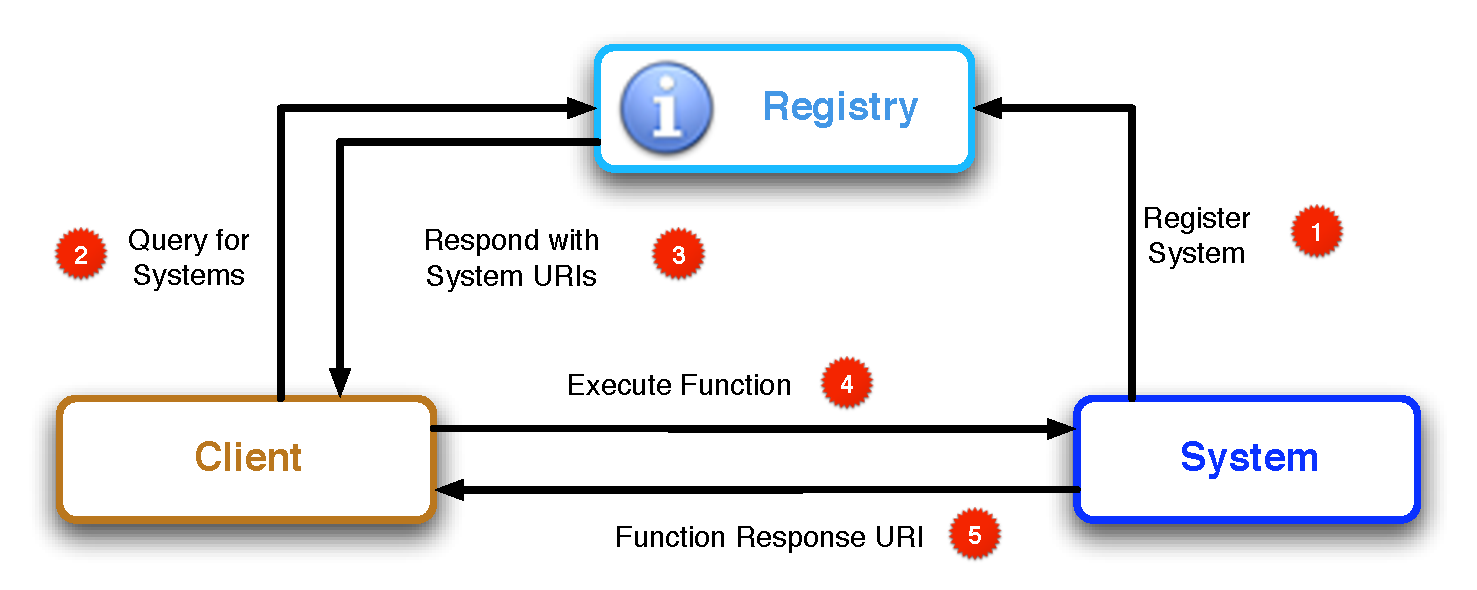
\includegraphics[width=0.70\textwidth]{./images/esp_overview.pdf}
  \caption{ESP framework operations overview.}
  \label{fig:espoverview}
\end{figure*}
\section{System Overview}
The overall architecture for the ESP Framework involves three main components. First, there is the actual system, which represents the sensor network that is being registered. 
The registry is the second element in the architecture and is the location where sensor systems are registered and where the user can actually query for systems.  Finally, there is the
client that accesses both the registry and the individual systems. Figure \ref{fig:espoverview} contains all the entities in the architecture and typical operations that can occur during
normal interaction.

In order to illustrate how the framework works in general, the usage scenarios will be described below.  

\begin{enumerate} \item \textbf{Register System}

During the registration process for a sensor, the first activity that needs to be performed is to create a ESPml document that describes the sensor network system as a whole.  This can be
done manually by an application developer or done automatically by analyzing the sensor system and generating the appropriate XML to represent the
system.  In addition, one must define all the functions that are described as being available in the ESPml document in the actual system.  Finally, the ESPml document must be sent to the
registry.  The process of sending information to the registry occurs through a web services interface where a method for registering the system is exposed.  At the actual registry, the
system ESPml is populated into a database.  More details about the database structure will be given in Section 5.

\item \textbf{Query for Systems}

In order to query for systems, the client sends a request to the registry with an area of interest.  The area is described as a polygon and the actual coordinates are encoded as a ESPml
document.  Again, there is a method exposed on the registry through web services that enables communication between the client and the registry to occur.

\item \textbf{Respond to Query}

After a request for sensor systems is sent, the registry responds to the client by sending back uniform resource identifiers (URIs) for the corresponding systems in the polygon area
submitted.  The actual response is an ESPml document that contains all sensors, platforms, and fields within the polygon. The URIs are addresses to the system's web service interfaces. 
Furthermore, descriptions for the different aspects of the system and the functions provided by these entities are detailed in the ESPml document.

\item \textbf{Function Execution Request}

Once the client gets back all the systems in a certain area of interest, a possible next step is to execute a method on the systems. In this 
case, a light weight version of the ESPml document, which contains only the URIs and the function to execute with any required variables filled in, is sent to the specific system.  
The systems have a web service exposed function to take in generic queries that are defined by the ESPml document.

\item \textbf{Function Response}

The final step in a typical interaction will be the actual system responding to the function execution request.  This occurs by the system returning a ESPml document that contains the
output tag for the function.  The output tag contains the name of the function, the return type for the result, and a URI that points to the result.

\end{enumerate}

Overall, the ESP framework is simple, yet robust enough to handle a wide variety of heterogeneous systems.  Furthermore, the use of ESPml and web services makes interoperable communication
possible in a standard fashion.  More details about each of the different parts of the architecture will be given in Section 5.


\section{ESPml Schema}

\subsection{Purpose and Goals}

The purpose of the ESPml schema language is to define a standard
protocol with which the different entities in the framework 
can communicate and also to have a unifying grammar that systems 
can describe their abilities. ESPml is held very generic such that it
can describe a lot of different systems like databases, sensor
networks, weather stations or even web cameras.

\subsection{Components}

The different components in ESPml describe the different parts of a
system. The main entity is the system element. The system element
contains one or more fields, which are a collection of one or more
platforms. And finally, a platform is a collection of sensors, the
smallest entity possible. We will now go into details of each of the
elements.

\subsubsection{System}
\begin{figure}[t]
  \begin{center}
    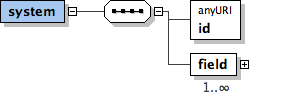
\includegraphics[width=0.33\textwidth]{images/system}
    \caption{Model view of the system component in the ESPml schema.}
    \label{fig:system}
  \end{center}
\end{figure}
Figure \ref{fig:system} depicts the model view of the top-level
element of the schema, the system component. The system consists of an
id element of type anyURI and one or more field elements. The id
element points to the address where the system's web services can be
reached, i.e., where one can execute remote functions through web
service calls. The field elements represent actual sensor
networks. For example, if a system has multiple physical deployments,
and there is one common interface for all the fields in the system,
then the different deployments can be represented as different
fields. We will describe the field element in the next section.


\subsubsection{Field}
\begin{figure}[t]
  \begin{center}
    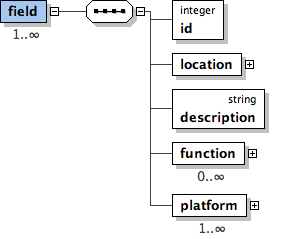
\includegraphics[width=0.39\textwidth]{images/field}
    \caption{Model view of the field component in the ESPml schema.}
    \label{fig:field}
  \end{center}
\end{figure}
Illustrated in Figure \ref{fig:field} is the field element of
ESPml. The field consists of an id of type integer. This id should be
unique within the system and is used to identify the field. The
location can be a point or a polygon which describes the physical
location of the field. We will describe the location element in more
detail in Section \ref{sec:location}. Each field has a description
element of type string which describes the type and purpose of the
field in a verbal manner. A field can also have zero or more functions
associated with it. In general, these functions should act on
the whole field, for example, they could return the average value of a
sensor reading over the whole field, etc. The last element in a field
is one or more platforms.


\subsubsection{Platform}
\begin{figure}[t]
  \begin{center}
    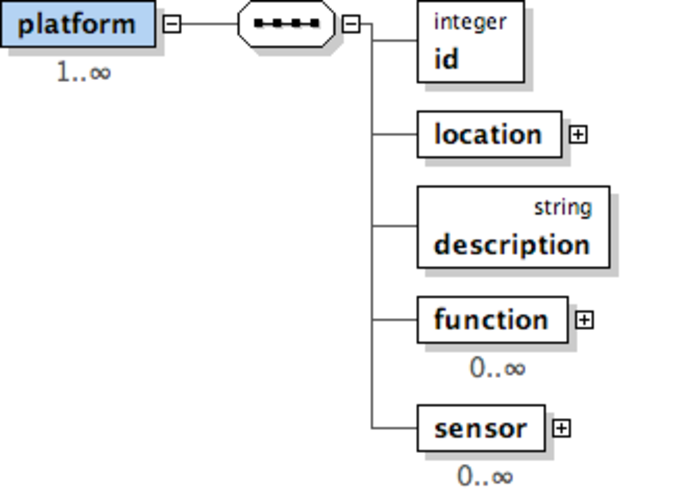
\includegraphics[width=0.39\textwidth]{images/platform}
    \caption{Model view of the platform component in the ESPml schema.}
    \label{fig:platform}
  \end{center}
\end{figure}
Figure \ref{fig:platform} shows the model view of the platform
element. A platform element represents a physical entity with a
micro-controller, some communication device and a possible energy
source. The integer id in a platform has to be unique within the
field. Thus, the field id and the platform id can uniquely identify
any platform in the system. Each platform has a location, a
string description, and functions which can be executed.  These functions can 
affect the
platform for actuation purposes, retrieve data values such as the exact
location, the local time at the platform, or to move the platform
around. Each platform also contains zero or more sensors.


\subsubsection{Sensor}
\begin{figure}[t]
  \begin{center}
    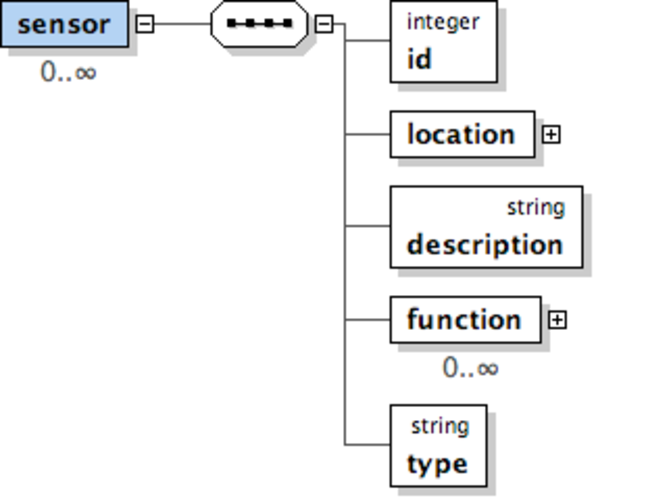
\includegraphics[width=0.39\textwidth]{images/sensor}
    \caption{Model view of the sensor component in the ESPml schema.}
    \label{fig:sensor}
  \end{center}
\end{figure}
Probably the most important component of the ESPml schemas is the sensor. 
Figure \ref{fig:sensor} depicts the model view. The sensor
element represents a sensor on a platform, such as a thermistor,
light-sensor, camera, etc. The id must be unique on the
platform. Similar to the other elements, the sensor element has a
location, description, and function element. One additional important
element is the type element which describes the type of sensor. This
type is not standardized right now, and can thus be defined by the system
developer.  This will change in the future since we intend to provide a standard for describing
sensor types.

\subsection{Descriptions}
The next four sections will explain the different additional fields
for the field, platform and sensor element in more detail. 

\subsubsection{Location}\label{sec:location}
The location element describes, as the name suggests, the location of
the enclosing element. The location is described either by a point or
a polygon element. The point element contains a simple string of the
format ``$latitude$, $longitude$, $altitude$'' and is derived from the
GML standard. The polygon is composed of a multi line string, where
each line represents a corner of the polygon and is also derived from
the GML standard. The format for each line is the same as the point
element. Additionally, the polygon has to be closed, i.e., the first
and last point have to coincide.

\subsubsection{Functions}\label{sec:function}
\begin{figure}[t]
  \begin{center}
    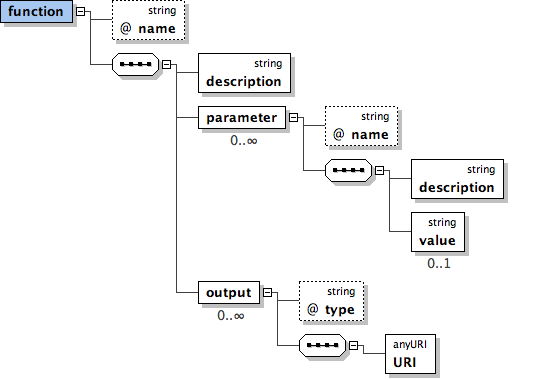
\includegraphics[width=0.49\textwidth]{images/function}
    \caption{Model view of the function element in the ESPml schema.}
    \label{fig:function}
  \end{center}
\end{figure}
The function element is a little bit more complicated than the other
elements.  The location of the function within the XML determines to
which component it is attributed to. For example, a function in the field
element should affect the whole field, whereas a function in a
platform element should affect only that platform.

Figure \ref{fig:function} depicts its model view. Each function has a
name attribute. The name attribute should be reflective of the
function's purpose. For example, a function which returns a sensor's
data, should be called \verb|getSensorData|, a function which sets the
sampling rate of a sensor, should be called \verb|setSamplingRate|,
etc. We do not enforce a naming schema for functions. Though we
encourage the user to choose meaningful names. In a later version we
will develop a standard naming schema for commonly used functions.

Each function element contains a description which
details what the function actually does. Additionally,
a function element contains zero or more parameter elements and zero or more
output elements. What role they play will be explained in the
following example where we show how one defines, executes and then collects the
data from a function.

\begin{itemize}
\item \textbf{Declaring a Function}

The function declaration is done in the system's XML schema file which
is sent to the registry. Each field, platform, and sensor should
define the functions it supports, including each function name
attribute, the description element, and the parameter elements with
name and description, which need to be provided to execute the
function later on. The following code example is an excerpt of a ESPml
XML file a system sends to the registry, and defines a sensor with
two functions. The first function gets the current sensor value and has no
parameter. The second function gets the average value over a certain number
of recorded data. Thus, it needs a parameter which tells the function
how many elements it should calculate the average.

\lstset{basicstyle=\small,breaklines=true}
\begin{lstlisting}
...
<sensor>
  <id>1</id>
  <location>
    <point>
      <pos>34.0682,-118.44,0.00</pos>
    </point>
  </location>
  <description>PhotoSensor</description>
  <function name="getCurrentValue">
    <description>Get the current value for this sensor.
    </description>
  </function>
  <function name="getAverageValue">
    <description>Gets the average for this sensor.
    </description>
    <parameter name="numberElements">
      <description>The number of elements for which the average should be calculated.
      </description>
    </parameter>
  </function>
  <type>Light</type>
</sensor>
...
\end{lstlisting}


\item \textbf{Executing a Function}

If a client wants to execute a function, then it sends a ESPml XML
file to the system's URI. In the XML file, the user will add the function
element that needs to be executed on a field, platform, or sensor. 
It is also possible to execute multiple functions in one
request. The following listing shows parts of a ESPml XML file which
a client sends to a system to execute functions. This excerpt will
execute \verb|getAverageValue| on platform 1, sensor 1 with a
parameter value of 10, and it will get the current value of platform
2's sensor 1.

\lstset{basicstyle=\small,breaklines=true}
\begin{lstlisting}
...
<platform>
  <id>1</id>
  <sensor>
    <id>1</id> 
    <function name="getAverageValue">
      <parameter name="numberElements">
        <value>10</value>
      </parameter>
    </function>
  </sensor>
<platform>
<platform>
  <id>2</id>
  <sensor>
    <id>1</id> 
    <function name="getCurrentValue">
    </function>
  </sensor>
<platform>
...
\end{lstlisting}

\item \textbf{Collecting Function Output}

The system will respond with another ESPml XML file which will be
filled with the output elements of the received function calls. The output
elements consist of a type attribute and a URI field. The type element
describes the mime-type of the file the URI points to. The following
listing is an example response to the function executed from the last
example. 


\lstset{basicstyle=\small,breaklines=true}
\begin{lstlisting}
...
<platform>
  <id>1</id>
  <sensor>
    <id>1</id> 
    <function name="getAverageValue">
      <output type="text/comma-separated-values">
        <URI>http://foobar.org:8080/sensor_getAverageValue/852760e7177ac9eeebcc16621ec2e83c
	</URI>
      </output>
    </function>
  </sensor>
<platform>
<platform>
  <id>2</id>
  <sensor>
    <id>1</id> 
    <function name="getCurrentValue">
      <output type="text/comma-seperated-values">
        <URI>http://foobar.org:8080/sensor_getCurrentValue/76344f22bdbc47211407b085bf5da147
	</URI>
      </output>
    </function>
  </sensor>
<platform>
...
\end{lstlisting}

\end{itemize}


\subsubsection{Mobility}
The location element has an optional element ``mobile''. This
indicates that the enclosing element is mobile and can move
around. This is an indicator that the location might not be the real
location where the element is right now and that one has to take some
precaution. In the future, we will require a special function to get
the enclosing elements exact current location if the mobile element is
defined.


\subsubsection{Additional Ideas}
The current ESPml schema is not complete and is open for further
development. It has all the functionality to get a simple example
system up and running but it will be extended in the future. Some
points which will be addressed are:
\begin{itemize}
\item standards for function names and types
\item confidentiality, privacy, and authentication
\item improved location element for different coordinate systems
\item scalability
\item etc.
\end{itemize}
We have a closer look at these extensions in Section \ref{sec:future_work}.

\section{Detailed System Design}
\begin{table*}
  \begin{center}
  \begin{tabular}{|l|llllll|}
    \hline
    \textbf{Name} & \textbf{Fields} & & & & &\\ \hline \hline
    System & id & systemURI & description & xml & & \\
    Field & id & systemId & fieldKey & xml & & \\
    Platform & id & fieldId & platformKey & xml & &\\
    Sensor & id & platformId & sensorKey & xml & &\\
    Location & id & referenceTable & referenceId & xml & & \\
    Polygon & id & locationId & xml & posList & &\\
    Point & id & locationId & xml & latitude & longitude & altitude \\
    \hline
  \end{tabular}
  \end{center}
  \caption{SQL Table Definitions for Registry Entries}
  \label{tab:registrysql} \end{table*} In addition to the ESPml schema language, the framework provides an architecture to
enable registration and interaction with sensor networks.  The basic two components involved in this prototype are the registry
and a system.  The following section details the design of these entities and goes over their interfaces.  

\subsection{Registry} 
The registry is the component that serves as a repository for sensor systems.  It provides services that
enables sensor systems to be added, updated, deleted, and queried for.  In terms of its architecture, one can think of it as a
database back-end with a web service front-end.  The sensor systems are registered by providing an ESPml document.  Thus, the
database structure is modeled similar to the hierarchy of the ESPml schema.  Table \ref{tab:registrysql} shows the definitions
of the various tables that are involved in storing a sensor system in the registry database.  One of the main aspects of the
database structure that needs to be pointed out is how locations, polygons, and points are represented.  Instead of storing them
as pure XML strings, the basic components of each of these structures are represented as fields in the tables.  This enables
efficient searching especially when location based queries are initiated on the registry.  To make the registry faster, a more
thorough design analysis of the database structure needs to be made and is marked for future work.

In terms of interfaces, the registry uses web services via SOAP to implement remote procedure calls.  The following functions are
exposed as part of the service: \verb|register|, \verb|unRegister|, \verb|update|, and \verb|listSystems|.  

\begin{itemize}

\item \textbf{register}

The register function takes an ESPml document that
describes a system and adds it to the database.  If there is already a system in the registry with the same identifier, 
then the old system will be deleted and the new one will be added.  

\item \textbf{unRegister}

In the unRegister case, again a ESPml document will be provided
as input, and the registry simply deletes the system described from the database.  

\item \textbf{update}

The update function is similar to sending the same system
twice via the register command.  The purpose is to update an existing entry.  If the entry does not exist, then it will be added.

\item \textbf{listSystems}

The listSystems function takes a low overhead ESPml document that contains a polygon area that is described as a point string.  The registry responds
with a ESPml document with all the systems, that are part of the polygon area.  

\end{itemize}
If there is a problem due to improper ESPml formatting or
inconsistencies exist in the actual call 
when compared to the database, then an error string is returned.  Standardization of the return value types needs to be made and this is considered an essential next step.

\subsection{System}

The system component represents the actual sensor system that client applications and other sensor systems can access.  Essentially,
the system component is a gateway to the sensor network as a whole.  Interactions with the sensor network occurs through a web service
interface named execute.  

\begin{itemize}

\item \textbf{execute}

Once a consuming program finds the appropriate system they want to interact with, the component runs the
execute command with an ESPml that specifies what functions to run on the system.  The result of the execute command is a lightweight ESPml document
that contains the output of the functions.  The output elements consist of the type attribute and a URI field.  The actual code necessary
to execute the function is defined by the individual sensor network.  Also, the availability of the output is also determined by the
sensor network.  
\end{itemize}
Overall, the framework dictates that the system needs to implement the functions that it specifies, provides a standard method
to actually interact with the system through the execute web service RPC call, and provides a standard way to format the response or output
for the execution.


\section{Evaluation} In order to evaluate the ESP framework, we created several systems that would be registered and also a geo-centric client that can actually query and interact with the
example systems. The following section details the different types of systems implemented and also the architecture of the client.

\subsection{Example Systems}
One of the main goals of the ESP framework was to be able to represent several different types of networked systems.  Furthermore, we wanted to have a low development overhead to use the
framework.  Currently, we provide a Python based system template that users can utilize to add their system in to the framework.  Essentially, a system would need an ESPml document describing its 
capabilities and must modify the system template to add the proper hooks for the functions that are specified in the ESPml description.

There are several systems that were added to the architecture to demonstrate its robustness.  The systems are shown visually as Figures \ref{fig:ui1}, \ref{fig:ui2}, and \ref{fig:ui3}.

\begin{itemize}
\item \textbf{Virtual Weather Stations}

In order to demonstrate that the ESP framework can handle many systems in terms of quantity, we added virtual weather stations for every zip code for a particular region.  In this case, it is 
for the state of California.  Essentially, a system for each zip code in the state was added to the registry with function capabilities to get the current weather information, a ten day forecast,
and an hourly forecast.  The results of running these functions results in a URI that represents a web page that contains the actual information about the weather forecasts.

\item \textbf{Community Web Cams}

Another type of system that was added using the ESP framework are web cams that exist already for community monitoring.  Specifically, we implemented three web cams in the Los Angeles region that
show pictures of UCLA, Santa Monica pier area, and Venice.  The systems have a function that gets the current picture of the region they are monitoring.

\item \textbf{Actuated Network Camera}

To demonstrate the ability to take parameters as part of a function call to a system, we implemented a Sony RZ30n network camera as a system.  Using the system, a user can set the pan, tilt, and
zoom values and then obtain either a picture or a movie.

\item \textbf{Photodiode Sensor Network}

Another capability that the ESP framework enables is aggregation functions through the use of platforms or fields.  A photodiode sensor gateway that operates over five MicaZ motes
is registered using the framework.  Not only can one get photodiode values from any of the individual motes, but one can also perform aggregation on the whole field to get an average value
for the photodiode readings.  Furthermore, one can set the individual sampling rate for any of the photodiode sensors.

\end{itemize}

\subsection{Client Application}

To interact with the ESP framework and also the systems that were implemented using the architecture, a geo-centric web client that relies on Google Maps was created.  Essentially, the 
user has the ability to draw a polygon box over a certain area and then query for all the different networked systems in that space.  When the results come back from the registry, the networked
systems in that area are represented as click-able point icons.  Different colors for the point icons represent the levels of abstraction for the systems.  For instance, fields are
represented as purple icons, while platforms and individual sensors are green and yellow. Once a user clicks on the icons, a box layer pops up that shows a description of the
entity that is being interrogated and then the user can interact with the component by clicking on buttons that represent function calls.  The results of the function call show up on a side
frame.  Overall, the client application provides a visual interface that users can use to interact with the sensor systems that are currently registered.

\subsection{Observations}

Based on implementing the various example systems with the framework and creating the client application, several observations were made.  While evaluating the speed of queries, we realized
that the database is a bottleneck.  We suspect that this is the case due to the fact that there needs to be some optimization techniques applied and the actual design of the database model needs to be
improved.  Another point that became clear is that for systems with numerous functions, a more robust interface then a window listing all the functions needs to be obtained.  Furthermore, we 
realized the limitations of the Google Map interface as we tried to map more advanced functionality onto it.  
There are situations when non-location based queries might be necessary and also the interface does not provide advanced mapping functions
such as temporal or spatial visualization overlays and analysis techniques.  Overall, there is a need for different types of client applications and also optimizations in the various parts
of the framework.


\section{Future Work} \label{sec:future_work}
There are a few different areas that should be investigated further
in terms of this project.  First, some additions need to be made to
the ESPml schema language in order to more accurately describe certain
types of systems.  Also, there are changes that need to be made to the
architecture in order to scale the platform as a whole.  Furthermore, there are
some issues related to privacy, authentication, and standardization
that need to be addressed.  Finally, some additional systems and clients need to
be made for the architecture that can act as services that other
components could use.
\subsection{Standardization}
One of the main actions that needs to be performed in terms of ESPml is
standardization of a few different aspects of the schema.  ESPml
allows different sensor types to be defined.  Currently, these types
can be any arbitrary name.  But there should be a standard naming
convention for the sensor types.  This will enable users that use the
framework to interpret the sensor types programmatically.
Furthermore, certain sensor types should have standard functions that
need to be defined.  These functions will have a certain prototype
associated with them and a standard output as well.  For instance, one
can expect all sensors that observe some type of phenomena and
quantify it in terms of a measurement to have a function to get the
current value.  In addition, they should be able to get the average
over a period of time and to set the sampling rate.  Having
this type of standardization will make describing sensors that are
similar easier since the same schema constructs can be repeated and
guarantee the end user certain basic functionality for most sensor
types.
\subsection{Mobility and Availability}
When describing sensor systems, two attributes that need to be
expressed in some fashion is mobility and availability.
Mobility deals with the notion of whether the system actually moves.  Since the ESPml
schema has a location tag as part of the description language, if the
systems are mobile then this location tag may not be reliable.  To
represent the difference between mobile systems and non-mobile
ones, a mobility tag can be added to different constructs of a system
to indicate that the location might not be reliable based on the information
in the registry.  At this point, the location that is in the actual ESPml
description serves as the last provided location by the sensor system
or the location that the sensor system is actually located at with the
highest probability.  In the next revision of the schema, a confidence
interval can be given to the location indicating how likely the node
will be at that particular location.  Also, if the mobile tag exists, a function
will be required to specify the exact location for that system.  

In terms of availability, one would introduce timestamps and a time to
live counter on the registry.  Basically, when a system is registered
it would be assigned a time to live in which the system is
required to re-contact the registry to verify that it is still
available.  The client program can then check the
registry to get the time to live requirement and at what time the
system last updated the registry to evaluate the availability
confidence level for a system.  Furthermore, statistics can be kept on
the registry about the quality of the system connection.
Overall, both mobility and availability are important aspects of a
sensor system that need to be addressed in the ESPml framework.

\subsection{Authentication and Confidentiality}

There are some key issues that need to be addressed for the ESP framework to
succeed that revolve around security.  Basically, the idea of
having certain services private, users authenticated, and keeping data
confidential are necessary.  There are several methods to address this
issue.  One can imagine creating a system in the actual ESP framework
that enables these attributes to be realized, but a better approach is
to leverage technologies that are already in the market that provide
similar capabilities.

Since ESP framework revolves around the web services platform, a
natural candidate that needs to be analyzed is web service security (WSS
or WS-Security) \cite{securews}.  Basically, WSS is a set of
enhancements to the SOAP messaging protocol in order to provide the
protection needed for authenticity, integrity, and confidentiality of
a message \cite{wss}.  In another words, WSS defines the structure for
SOAP that enables these properties to take place in the actual message
document and for the actual functionality that is provided.  Using XML
Signatures to sign data provides integrity.  XML Signatures contains a
section which has information about the signature algorithm used,
canonicalization method used, the digest value, and key values.  By
checking the signature one can determine if the actual messages
between various sources has been tampered in some fashion.  Confidentiality
is provided by employing encryption techniques under the standards of
XML Encryption. The elements of the SOAP message are
encrypted instead of in plain text.  Finally, authenticity can be
provided by using a key management scheme that can be provided by the
registries.  The registries would provide the public and
private key infrastructure and manage keys for systems and clients
that need to use those systems.  Private keys are kept a secret and
public keys are distributed freely.  The registries could generate the
key pair for each of the different clients that would want to use a
system.  The actual system can then send the message to the registry
to authenticate using a certain method and then a secure connection could
be established between the client and system since there will be a
direct connection.  Also, restrictions related to who and to what capacity
the functions are exposed can be boot strapped through this key management
protocol

In addition to digital signatures, encryption methods, and key management
methods, there also exists policy languages for web services.  This includes
XACML and SAML standards that provide an authorization framework \cite{godik:oea}.  In this
type of model there exists a PEP (Policy Enforcement Point), PDP (Policy
Decision Point), PIP (Policy Information Point), and PAP (Policy Administration
Point).  The PEP takes a request from a client and sends the request to the PDP.
The PDP then gets policies from the PAP and gets attributes using the PIP concerning
the subject, the resource, and the environment and makes a decision for the request.
The request is sent back to the PEP from the PDP and then conveyed to the user.

Clearly, there needs to be more investigation in this space to make a
system that would work correctly for a framework of this type.
Overall, previous work in this area will serve as inspiration in
order to come up with a scheme that will be effective.

\subsection{Selective Sharing and Verification}

Issues related to providing capabilities such as selective sharing and
verification of certain information adds an extra dimension to the ESP
framework.  Selective sharing refers to the idea of providing
different services or outputting various granularity of data
depending on the client that is actually querying for the service.
This can be done on the systems themselves, but as scale gets higher,
one can imagine mediators between the clients and the actual systems
performing this type of action.  Also, in addition to selective
sharing, the concept of verifying certain aspects of the system is an
interesting idea to consider.  For instance, if the framework provided
a method to verify the location of a sensor system and attach a
confidence level associated with this index, then this would be useful
for client applications. One can imagine mediators being involved in
storing or providing this information in some form.

\subsection{Scalability} 

As more sensors are added and query requirements diversify,
scalability becomes an issue with the ESP framework.  Managing a
large amount of sensors with one registry is not feasible without
having performance issues related to queries and management.  Thus, a
hierarchy for registries needs to be developed.  The Domain Name
System (DNS) platform can be used as an example model
\cite{mockapetris:ddn}. When a system is registered, a unique name
could be provided to the system.  An example naming scenario would be to
adopt the unique name based on how domain names are formatted. Thus,
there will be top level domains and then sub domains associated with
sensors that are somehow related.  For instance, sensor systems
located in the same region might share a certain level in the
naming convention.  Then, the actual registries could be arranged in a
tree fashion where each registry is responsible for a certain zone of
entries.  There would be a a set of root registries that handle the
top-level construct in the naming convention.  If the query that comes
cannot be addressed by the top-level registry then the request
would be passed along the hierarchy to a registry that can actually
handle the request.

In terms of queries, location is the only aspect that can be
searched for in terms of finding systems.  But one can imagine other
querying methods.  For instance, the type of sensor, functionality of
sensor systems, and a common naming convention can all be attributes
that can be queried for by clients.  These types of searching
capabilities for sensor systems need to be incorporated into the
registry to make it usable by a larger set of clients.

\subsection{Client Applications and Systems} 

Currently, there are many different types of network systems
that are incorporated into the ESP framework.  But there are not many
clients that use the actual system.  An example Google Map client
interface is provided that enables searching and 
interactivity through a map interface, but one can imagine a larger
plethora of services that can be created on the client side.  Some
necessary clients include a database archiving entity that takes and
stores readings from various sensors that are registered in the ESP
system.  The actual archiver then could add itself as a system
that other clients could actually interact with if needed.  There are
also more sophisticated analysis services that can be provided as
clients by using the capabilities of popular statistical and signal processing 
software components such as R, ESRI, and Matlab.  Finally, we can imagine
using Google Earth or other mapping tools to serve as
further client programs for users to visually query and interact with
various components in the system.


\section{Conclusion}
One of the fundamental characteristics of networks systems, especially sensor networks, is that they are heterogeneous in nature.  With the ESP
framework, we provided a standard method to manage, query, and interact with these varied sensor systems.  ESPml serves
as the model for describing sensor network systems at different levels of granularity.  The ESP architecture, which
includes a registry and system entities, uses
a web service based framework for locating sensor systems and then methods to actually interact with the systems themselves
including getting information and running specific functions.  A geo-centric web interface is provided as a portal for users
to interact with the various sensor systems that are available on the framework as well.


\section{Acknowledgments}
Thanks goes to Dr. Estrin and Dr. Srivastava for their help throughout the quarter while we progressed on our project.
Their guidance, enquiries, and challenges enabled us improve on the overall system and carefully make design decisions
as the framework was designed.  Furthermore, we appreciate the help of members of the Networked and Embedded System Laboratory
for inspiration on various topics and for entertaining various discussions about the project as a whole.

\bibliographystyle{unsrt}
\bibliography{report}
\balancecolumns\newpage\ \\\newpage
\appendix
\section{Source Code Structure}


The source code for the ESP framework is organized as follows.

\begin{itemize}

\item \textbf{Registry}

The code for the registry is under the "registry" directory.  config.py contains information regarding the SQL database connection attributes including the username, password, and database
name.  difdbi.py contains helper functions to add various components of a ESPml document to the database.  registry.py contains the SOAP server implementation that has all the interfaces
defined and then calls the appropriate functions to interact with the database.  registry\_client.py is a sample client that can test the registry.

\item \textbf{XML}

All the XML files associated with the ESP framework is stored in the XML directory.  espml.py, espmlsubs.py, and query.py are XML parsing utilities that help in representing a ESPml
document in terms of python objects.  The actual schema is named espml.xsd and an example system is named system1.xml.  Examples of ESPml queries and responses are presented as
locationQuery.xml and query\_response.xml. 

\item \textbf{Web Client}

The files that represent the geo-centric client are in the web directory.  index.html contains all the Java Script code to represent the Google Map and also interact with the map.  createHTML.py
actually makes queries and gets the response to them which the Java Script can use to display on the Google Map.  callFunction.py is a SOAP client that actually makes the web services calls to 
a system.  baseFunctionCall.xml is a template used to make function calls.

\item \textbf{System}

The files representing the base system and all the example network systems designed for this project are in the system directory.  system.py is a template for a typical network system. 
The rest of the files associated with each unique network system are under their corresponding directory name.  These include such things as sonycam, iTunes, beachCams, weather, and sos.

\end{itemize}

\begin{figure}[b]
  \begin{center}
  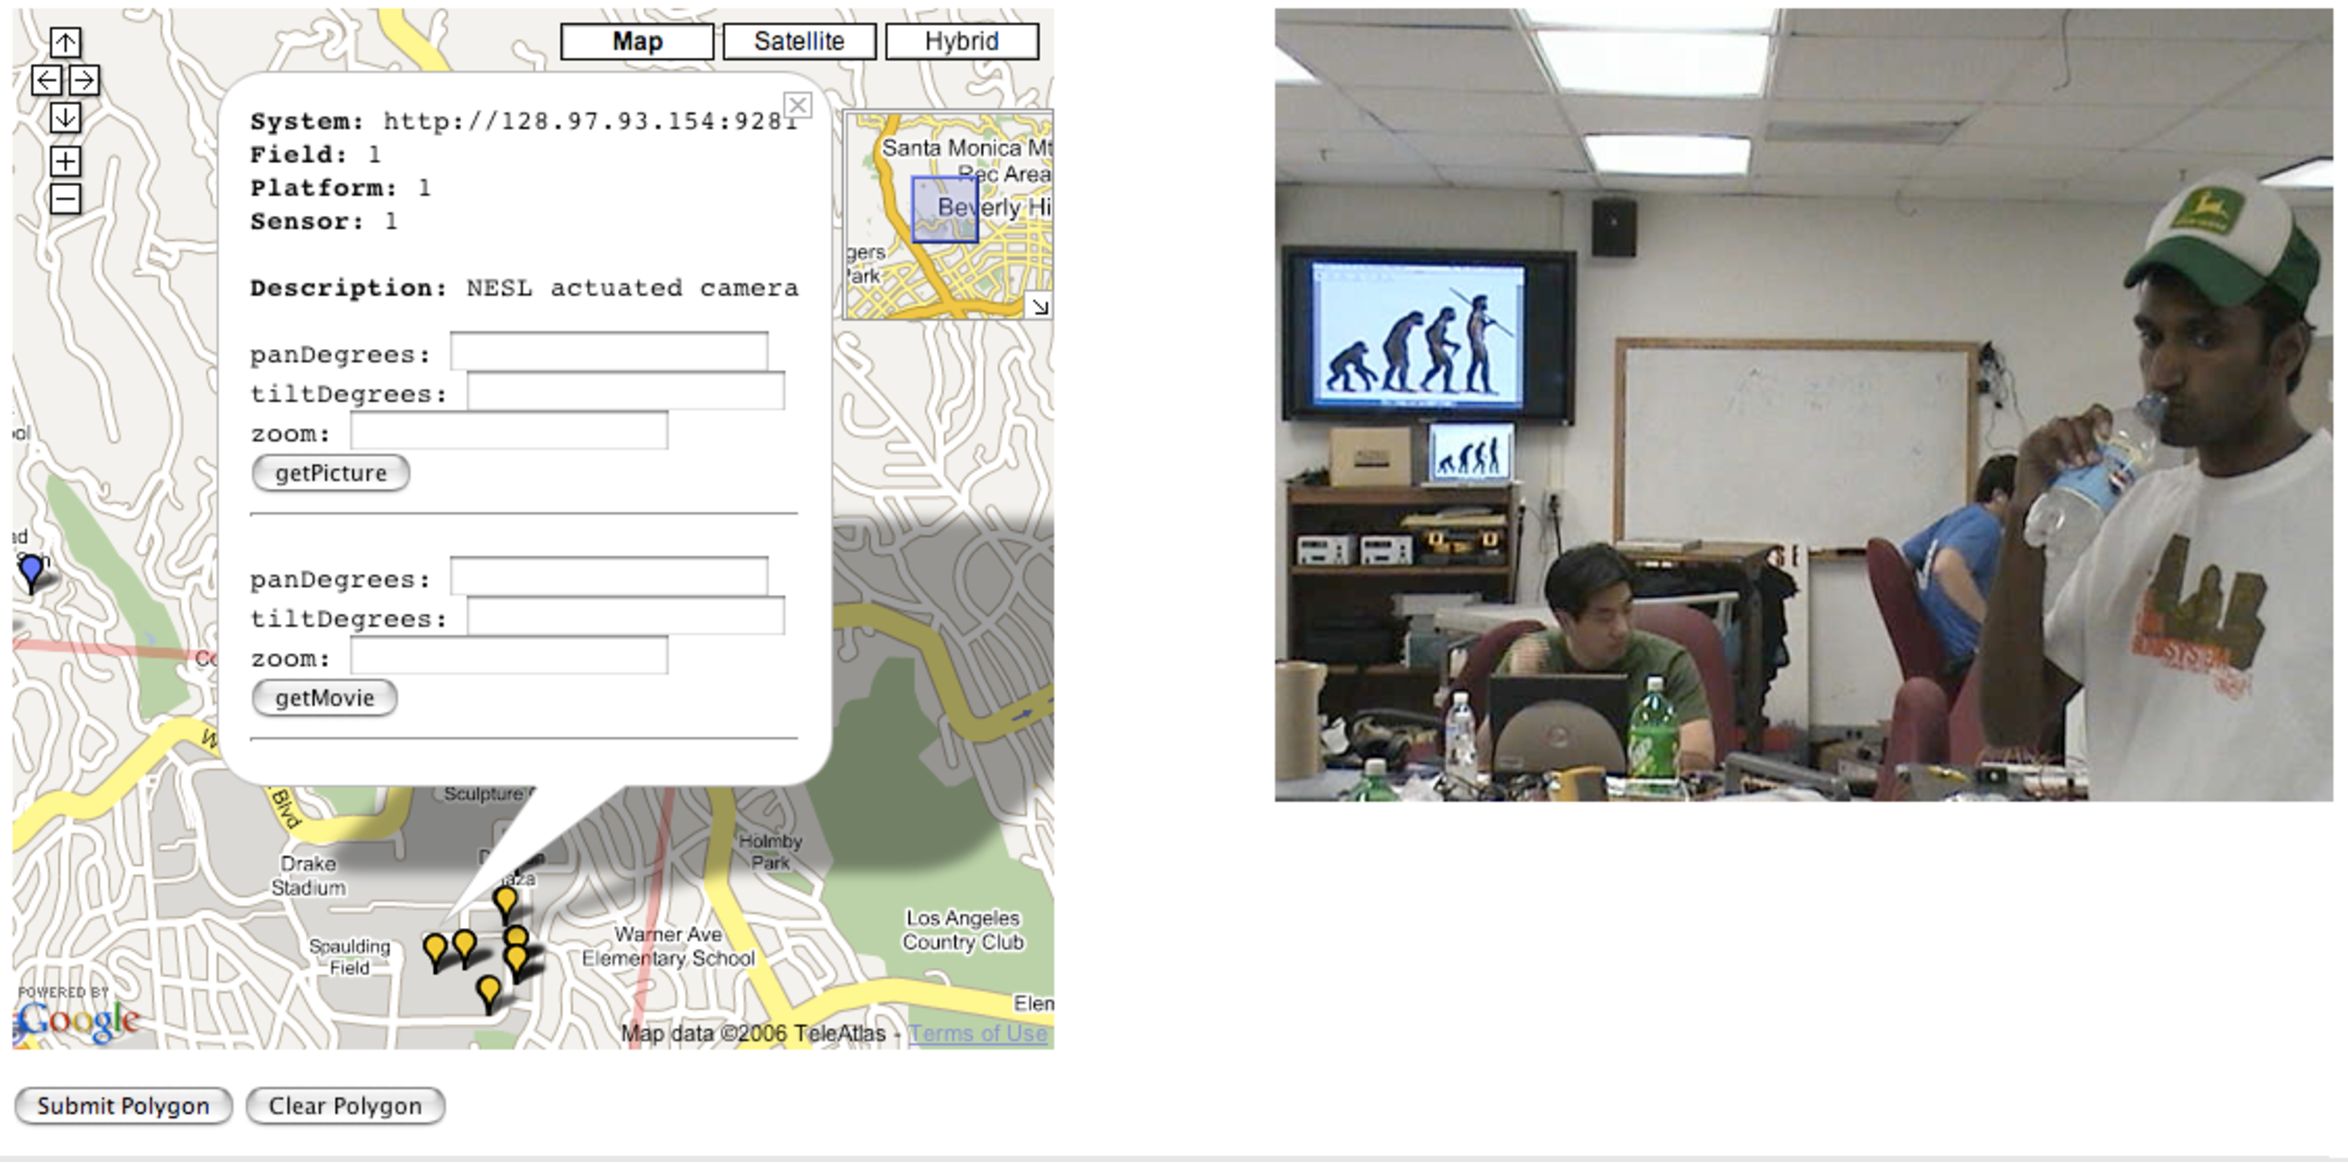
\includegraphics[width=0.49\textwidth]{images/ui1}
  \caption{Screen-shot of the Google Maps client and an actuated camera.}
  \label{fig:ui1}
  \end{center}
\end{figure}

\begin{figure}[h]
  \begin{center}
  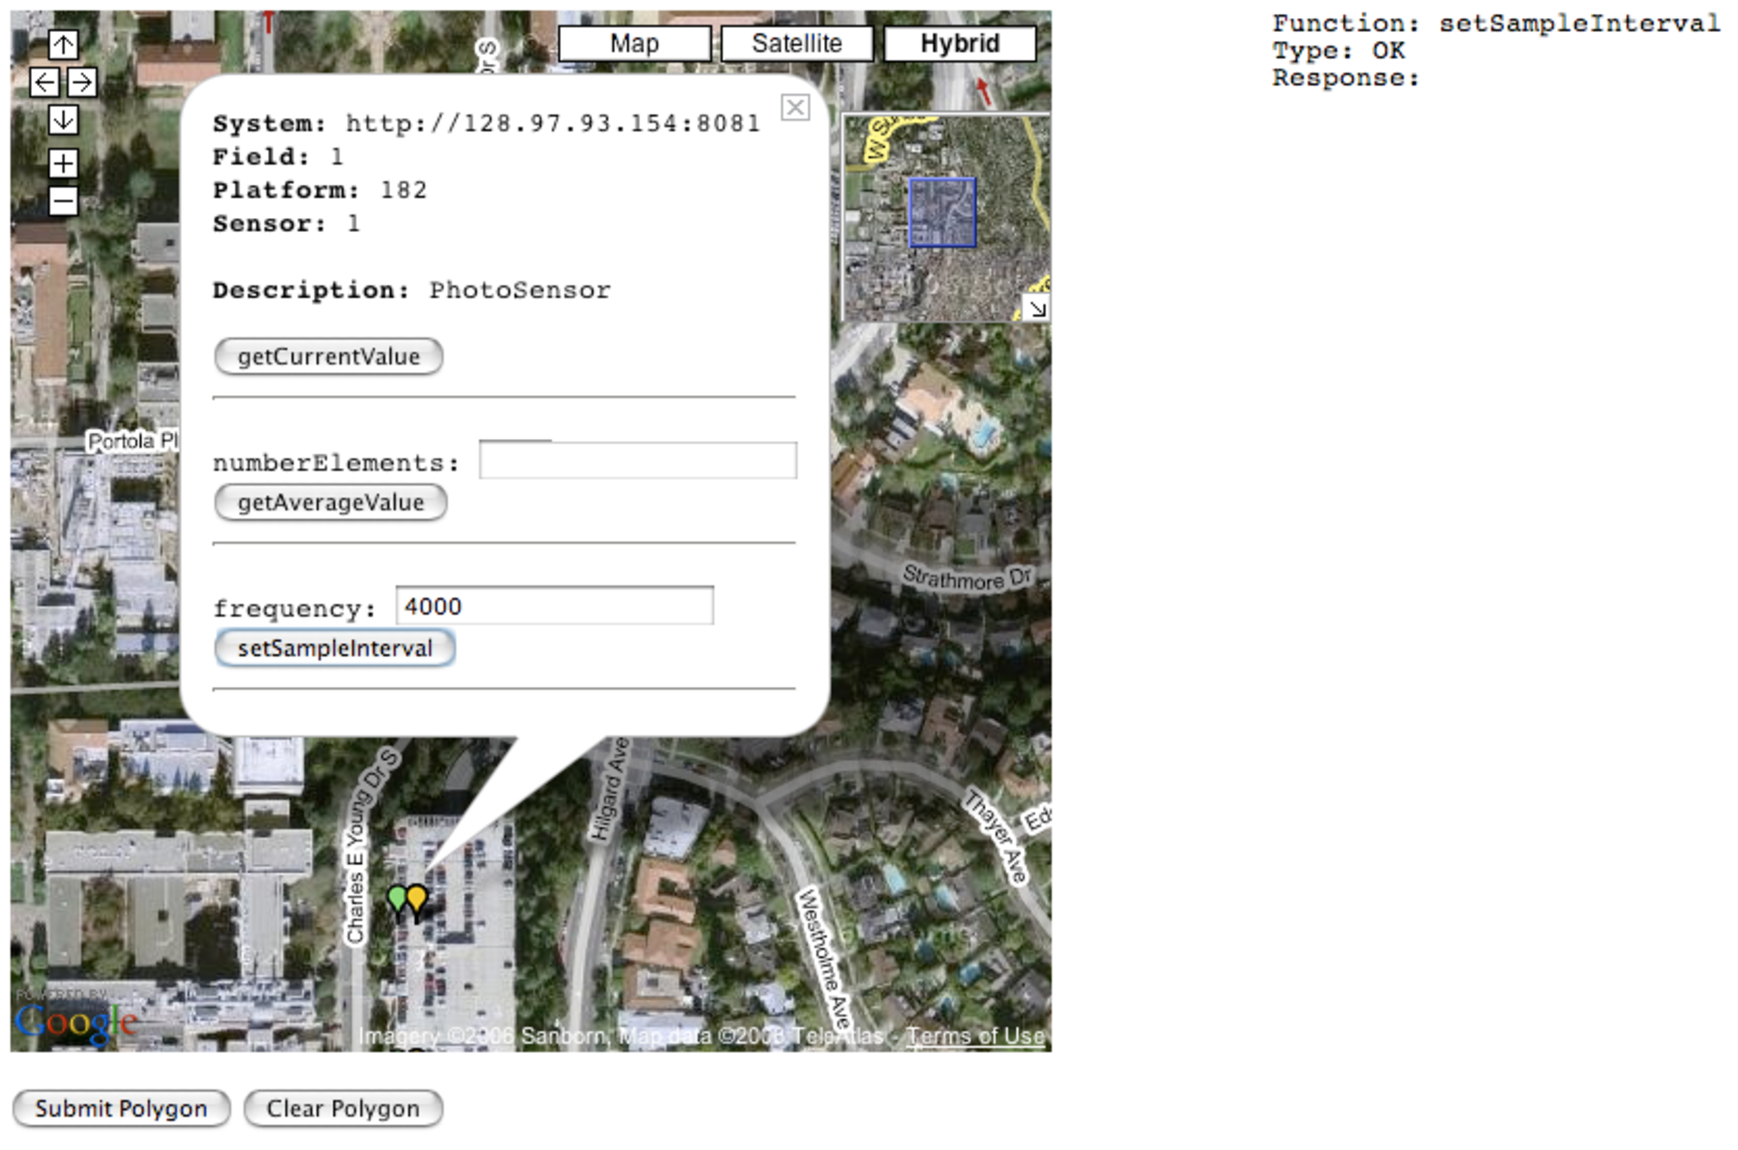
\includegraphics[width=0.45\textwidth]{images/ui2}
  \caption{Screen-shot of the Google Maps client and a small sensor
  network node's photodiode sensor.}
  \label{fig:ui2}
  \end{center}
\end{figure}

\begin{figure}[b!]
  \begin{center}
  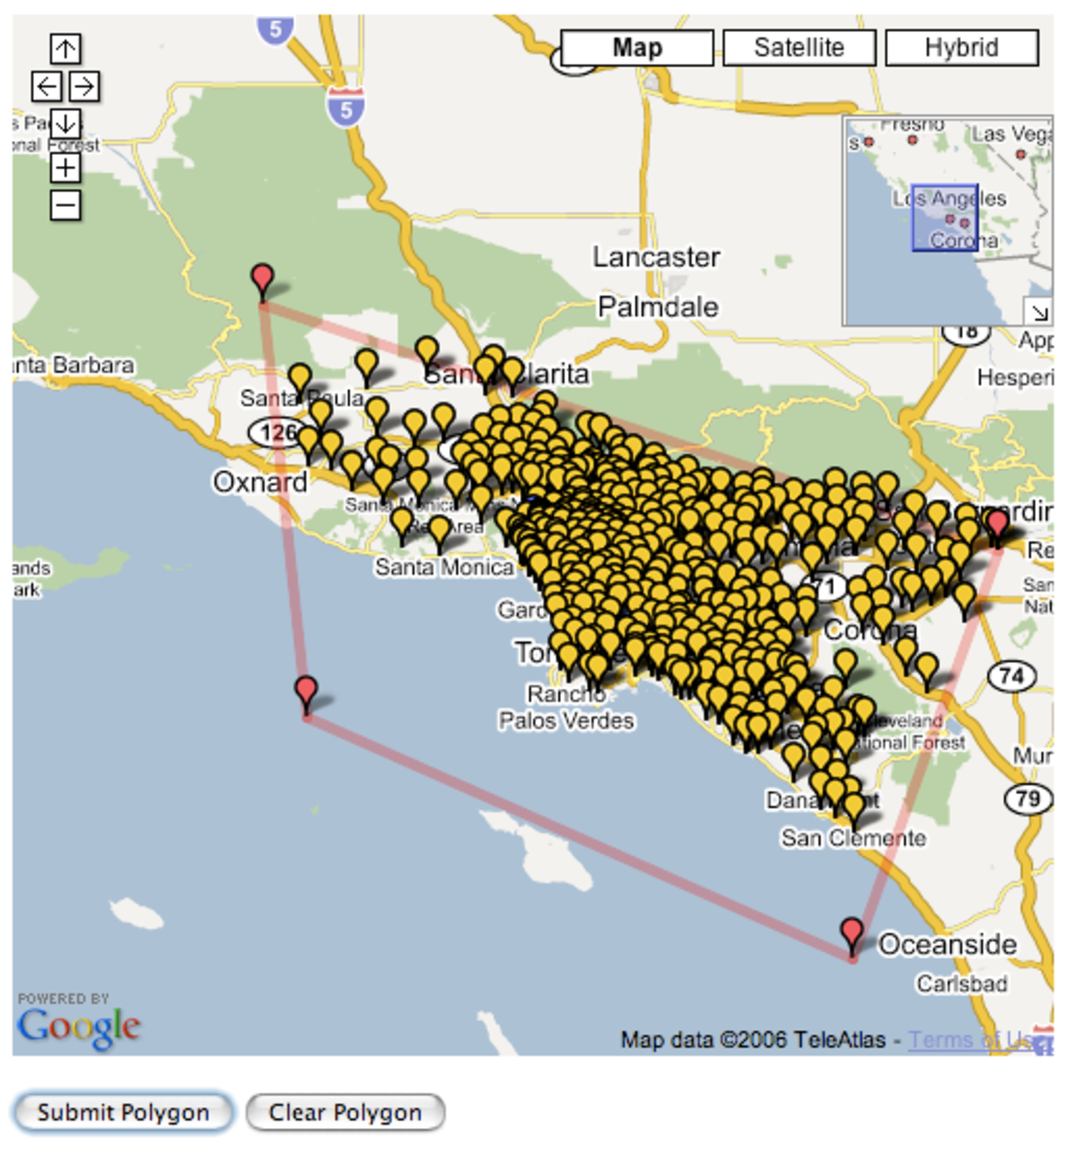
\includegraphics[width=0.35\textwidth]{images/ui3}
  \caption{Screen-shot of the Google Maps client and the weather
  stations in the Los Angeles area.}
  \label{fig:ui3}
  \end{center}
\end{figure}

\section{UI Examples}
Figures \ref{fig:ui1}, \ref{fig:ui2}, and \ref{fig:ui3} depict screen-shots of the
Google Maps client interface.



\section{ESPml Schema}
Figure \ref{fig:espml_schema} shows the ESPml schema as of writing
this report. Note that the schema is under development and might have
changed. Please contact the authors if you are interested in
the latest version.

\begin{figure*}[h]
\lstset{basicstyle=\tiny,breaklines=true}
\begin{lstlisting}
<?xml version="1.0" encoding="UTF-8"?>
<xs:schema xmlns:xs="http://www.w3.org/2001/XMLSchema">
    <xs:element name="system">
        <xs:complexType>
            <xs:sequence>
                <xs:element name="id" type="xs:anyURI"/>
                <xs:element name="field" minOccurs="1" maxOccurs="unbounded">
                    <xs:complexType>
                        <xs:sequence>
                            <xs:element ref="id"></xs:element>
                            <xs:element ref="location"></xs:element>
                            <xs:element ref="description"></xs:element>
                            <xs:element ref="function" minOccurs="0" maxOccurs="unbounded"></xs:element>
                            <xs:element name="platform" minOccurs="1" maxOccurs="unbounded">
                                <xs:complexType>
                                    <xs:sequence>
                                        <xs:element ref="id"></xs:element>
                                        <xs:element ref="location"></xs:element>
                                        <xs:element ref="description"></xs:element>
                                        <xs:element ref="function" minOccurs="0"
                                            maxOccurs="unbounded"/>
                                        <xs:element name="sensor" minOccurs="0" maxOccurs="unbounded">
                                            <xs:complexType>
                                                <xs:sequence>
                                                  <xs:element ref="id"></xs:element>
                                                  <xs:element ref="location"></xs:element>
                                                  <xs:element ref="description"/>
                                                  <xs:element ref="function" minOccurs="0" maxOccurs="unbounded"/>
                                                  <xs:element name="type" type="xs:string"/>
                                                </xs:sequence>
                                            </xs:complexType>
                                        </xs:element>
                                    </xs:sequence>
                                </xs:complexType>
                            </xs:element>
                        </xs:sequence>
                    </xs:complexType>
                </xs:element>
            </xs:sequence>
        </xs:complexType>
    </xs:element>
    <!-- Simple element definitions -->
    <xs:element name="id" type="xs:integer"/>
    <xs:element name="description" type="xs:string"/>

    <!-- Complex element definitions -->
    <xs:element name="function">
        <xs:complexType>
            <xs:sequence>
                <xs:element name="description" type="xs:string"></xs:element>
                <xs:element name="parameter" minOccurs="0" maxOccurs="unbounded">
                    <xs:complexType>
                        <xs:sequence>
                            <xs:element name="description" type="xs:string"></xs:element>
                            <xs:element name="value" minOccurs="0" maxOccurs="1" type="xs:string"></xs:element>
                        </xs:sequence>
                        <xs:attribute name="name" type="xs:string"/>
                    </xs:complexType>
                </xs:element>
                <xs:element name="output" minOccurs="0" maxOccurs="unbounded">
                    <xs:complexType>
                        <xs:sequence>
                            <xs:element name="URI" minOccurs="1" maxOccurs="1" type="xs:anyURI"></xs:element>
                        </xs:sequence>
                        <xs:attribute name="type" type="xs:string"/>
                    </xs:complexType>
                </xs:element>
            </xs:sequence>
            <xs:attribute name="name" type="xs:string"/>
        </xs:complexType>
    </xs:element>

    <xs:element name="location">
        <xs:annotation>
            <xs:documentation>Point: Specify three values representing x,y,z coordintes.</xs:documentation>
            <xs:documentation>Polygon:  Must be four pairs of x,y,z coordinates with last being identical to the first..</xs:documentation>
        </xs:annotation>
        <xs:complexType>
            <xs:sequence>
                <xs:element name="Mobile" minOccurs="0" maxOccurs="1"></xs:element>
                <xs:choice>
                    <xs:element name="point" minOccurs="1" maxOccurs="unbounded">
                        <xs:complexType>
                            <xs:sequence>
                                <xs:element name="pos" type="xs:string"/>
                            </xs:sequence>
                        </xs:complexType>
                    </xs:element>
                    <xs:element name="polygon" minOccurs="1" maxOccurs="unbounded">
                        <xs:complexType>
                            <xs:sequence>
                                <xs:element name="poslist" type="xs:string"/>
                            </xs:sequence>
                        </xs:complexType>
                    </xs:element>
                </xs:choice>
            </xs:sequence>
        </xs:complexType>
    </xs:element>
    <xs:element name="query">
        <xs:complexType>
            <xs:sequence>
                <xs:element ref="system" minOccurs="1" maxOccurs="unbounded"></xs:element>
            </xs:sequence>
        </xs:complexType>
    </xs:element>
</xs:schema>

\end{lstlisting}
\caption{ESPml schema used in the framework.}
\label{fig:espml_schema}
\end{figure*}


\section{ESPml Examples}
Figure \ref{fig:espml_example} shows an example for an ESPml document
which would be sent to the registry. It consists of three platforms
with id's 1, 182, and 196. Platform 1 has no sensors nor
functions. Platform 182 and 196 are equivalent and have one
photosensor connected. There are definitions for functions which act
on the field, or on the individual sensors themselves.

\begin{figure*}
\lstset{basicstyle=\tiny,breaklines=true}
\begin{lstlisting}
<?xml version="1.0" encoding="UTF-8"?>
<system xmlns:xsi="http://www.w3.org/2001/XMLSchema-instance"
 xsi:noNamespaceSchemaLocation="../../xml/espml.xsd">
 <id>http://foobar.com:8081</id>
 <field>
  <id>1</id>
  <location>
   <polygon>
    <poslist>34.0815,-118.46,0.00 34.0518,-118.46,0.00 34.0509,-118.42,0.00 34.0805,-118.42,0.00
     34.0815,- 18.46,0.00</poslist>
   </polygon>
  </location>
  <description>This is a small test field of SOS nodes.</description>
  <function name="getCurrent">
   <description>Returns the current values for all platforms in this field.</description>
  </function>
  <function name="average">
   <description>Returns the average over all platforms in this field. </description>
  </function>

  <platform>
   <id>1</id>
   <location>
    <point>
     <pos>34.0689,-118.44,0.00</pos>
    </point>
   </location>
   <description>MicaZ Basestation connected to the gateway.</description>
  </platform>

  <platform>
   <id>182</id>
   <location>
    <point>
     <pos>34.0689,-118.44,0.00</pos>
    </point>
   </location>
   <description>MicaZ node with Mica Sensor Board.</description>
   <sensor>
    <id>1</id>
    <location>
     <point>
      <pos>34.0689,-118.44,0.00</pos>
     </point>
    </location>
    <description>PhotoSensor</description>
    <function name="getCurrentValue">
     <description>Get's the current value for this sensor. </description>
    </function>
    <function name="getAverageValue">
     <description>Gets the average for this sensor. </description>
     <parameter name="numberElements">
      <description>The number of elements for which the average should be calculated. </description>
     </parameter>
    </function>
    <function name="setSampleInterval">
     <description>Sets the sampling frequency for this sensor. </description>
     <parameter name="frequency">
      <description>The frequency at which the sensor should sample. </description>
     </parameter>
    </function>
    <type>Light</type>
   </sensor>
  </platform>

  <platform>
   <id>196</id>
   <location>
    <point>
     <pos>34.0682,-118.44,0.00</pos>
    </point>
   </location>
   <description>MicaZ node with Mica Sensor Board.</description>
   <sensor>
    <id>1</id>
    <location>
     <point>
      <pos>34.0682,-118.44,0.00</pos>
     </point>
    </location>
    <description>PhotoSensor</description>
    <function name="getCurrentValue">
     <description>Get's the current value for this sensor. </description>
    </function>
    <function name="getAverageValue">
     <description>Gets the average for this sensor. </description>
     <parameter name="numberElements">
      <description>The number of elements for which the average should be calculated. </description>
     </parameter>
    </function>
    <function name="setSampleInterval">
     <description>Sets the sampling frequency for this sensor. </description>
     <parameter name="frequency">
      <description>The frequency at which the sensor should sample. </description>
     </parameter>
    </function>
    <type>Light</type>
   </sensor>
  </platform>

 </field>
</system>
\end{lstlisting}
\caption{Example for an ESPml XML document which would be sent to the
registry.}
\label{fig:espml_example}
\end{figure*}





\end{document}

